\chapter{Implement}
In this section, some examples of RMPs as well as implement detail are presented.
\section{Collision Avoidance}
A collision avoidance behavior task can be defined in 1D distance space, we denote the distance between two nearest points of interest as $d(t)$, thus, the state of distance space $x = d(t)$.
The cost or potential energy in GDS can be defined as $\Phi(x) = \frac{\alpha}{x^4}$. Then the "repulsive force" to push the robot away from the obstacle is $\nabla\Phi(x)=-4{\alpha}\frac{1}{x^5}$, where $\alpha$ is a constant gain. A naive but reasonable design of GDS can be given by set the second order dynamic system as 
\begin{equation}
\ddot{x} = - 4\frac{\alpha}{x^5}
\end{equation}
which can be seen as a system with constant inertia matrix $m = 1$ with non damper.  The phase portrait is shown as below.

\begin{figure}
\centering
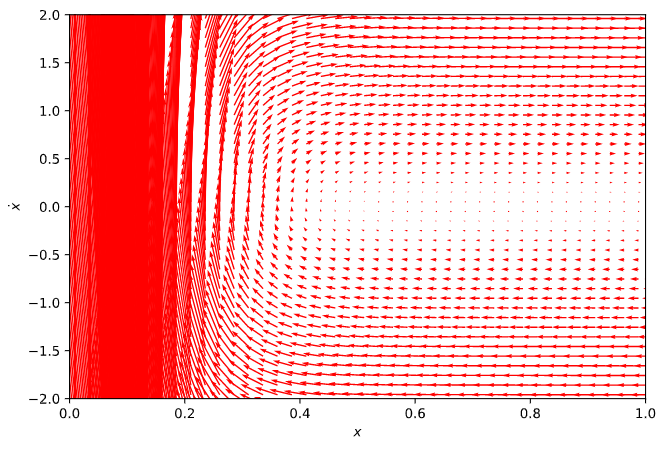
\includegraphics[width=0.55\textwidth]{Images/Chapter5/phase_portrait_obs_naive.png}
\caption{Phase Portrait of naive obstacle avoidance GDS}
\label{fig:chapter5_phase_portrait_obs_naive}
\end{figure}

Here in the figure, state $\yb = [x, \dot{x}]^T$ of this GDS is discretized, and each state corresponds to an arrow that indicates $\yd = [\dot{x}, \ddot{x}]^T$. We shall see that no matter how large the value $\dot{x}$ is, the vertical components of the arrows is the same with a certain value of $x$ , and the collision avoidance only "activates" when the robot is extremely closed to the obstacle and instantly push the robot away from this "barrier". 

\begin{figure}
\centering
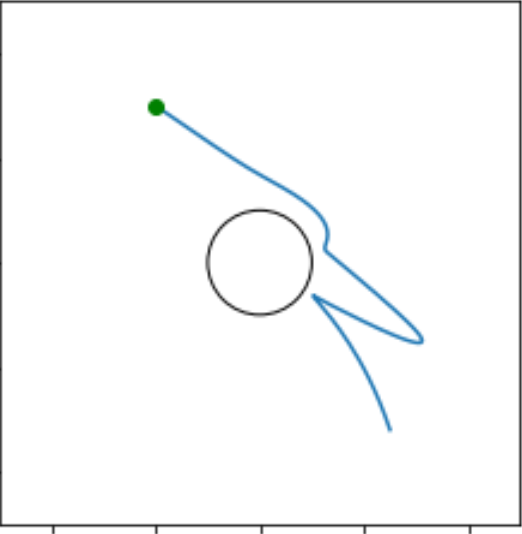
\includegraphics[width=0.55\textwidth]{Images/Chapter5/sim_obs.png}
\caption{Simulation of naive obstacle avoidance behavior}
\label{fig:sim_obs}
\end{figure}

To demonstrate this dynamic behavior, we simulate this collision avoidance and combined it with a target attraction task. The result is shown in 

Indeed, one could choose a mild behavior, for example, let $\Phi(x) = \frac{\alpha}{x}$, however  the stationary point may be unexpected  because this control law always generates a large "force" even if the robot in a relatively safe distance to the obstacle.





